\documentclass[12pt]{article}
\usepackage{amsmath}
\usepackage{tikz}
\usepackage{caption}
\usepackage{subcaption}
\usepackage[hidelinks]{hyperref}
\usepackage{cleveref}
\usepackage{amssymb}


\newcommand{\Price}[2]{P(#1,#2)}
\newcommand{\Ptotal}[1]{P(#1)}



\newtheorem{theorem}{Theorem}
\newtheorem{proposition}{Proposition}
\newtheorem{definition}{Definition}
\newtheorem{corollary}{Corollary}
\newtheorem{lemma}{Lemma}
\newtheorem{proof}{Proof}

\title{Bachelor Thesis}
\author{Alex Marek}
\date{\today}

\begin{document}
	
	\maketitle
	
	\section{Basic notions}
				
	\subsection{Introduction to graph theory}
		Graph theory is considered a relatively young mathematical discipline. Its official beginning is often associated with the first monograph on graph theory, written by Dénes Kőnig in 1936. However, the origins of graph theory date 200 year back, when in 1736 Leonhard Euler published paper, that is regarded as the first paper in the history of graph theory. In this paper, Euler addressed the famous problem of walking through all the bridges of the city of Königsberg without crossing any bridge more than once. Euler represented the map of city and its bridges as a graph, topology and theory that he had done has shown it's importance much later, in various fields, including for example traffic planning, computer science or electrical engineering. More importantly it laid the groundwork for a new branch of mathematics, graph theory.
		
		From the perspective of graph theory, a graph is a mathematical structure consisting of a set of objects (vertices) and connections (edges) between these objects.
 		Graphs can represent various real-world structures, from maps of cities connected by roads to electrical networks connecting sockets.
		Formally, a graph is defined as ordered pair \( G = (V, E) \), where \( V \) is a set of vertices, and \( E \subseteq \{\{v_i, v_j\} : v_i, v_j \in V\} \) is a set of edges, pairs of vertices.
		
		If we take a subset of the vertices of given graph, along with some or all of the edges between them we get subgraph. A subgraph of a graph \( G = (V, E) \) is a graph \( G' = (V', E') \) such that  
		\[
		V' \subseteq V \quad, \quad E' \subseteq E \cap \left\{ \{u,v\} \mid u,v \in V' \right\}.
		\]
			
		Edges in a graph can be either directed or undirected. A graph with directed edges is called a directed graph. In such a graph, each edge has an assigned direction from one vertex to another, we will not go into detail, as all graphs considered in this work are undirected. In an undirected graph, all edges are unordered pairs of vertices, undirected edges, representing symmetric relationships. Unless stated otherwise, consider all graphs in this work undirected.
		To understand next basic property of graphs, connectivity, we need to define term path. A path in a graph is a finite or infinite sequence of edges which joins a sequence of vertices, all of which are distinct. A graph is said to be connected if there exists a path between every pair of vertices. In contrast, a disconnected graph contains at least two vertices between which no path exists. This means the graph consists of two or more separate parts, called connected components. 
		We will refer to two vertices connected by an edge as adjacent, and the degree of a vertex is defined as the number of vertices adjacent to it(i.e., number of times it occurs in set of edges). In this context, a path can also be seen as a sequence of adjacent vertices, each of which appears at most once.
	
	\subsection{Weighted graphs}	
		In many applications, it is useful to associate a numerical value, called a weight, with each edge of a graph. For example, when modeling traffic, the vertices may represent cities and the edges represent roads, while the weight corresponds to the time required to travel from one city to another. 
		A weighted graph is a triple \( G = (V, E, w) \), where \( (V, E) \) is a graph and \( w : E \to \mathbb{R} \) is a weight function that assigns a real number to each edge. 
		In such graph, distance between two vertices \( u, v \in V \), denoted \( d_G(u,v) \),  is defined as the length of the shortest path between \( u \) and \( v \) in \( G \), it is computed as sum of the weights of edges along that path. Let us mention that if the graph is not weighted then usually distance is computed in the same way, with the only difference being that each edge is considered to have weight 1, i.e., \( d_G(u,v) \) equals the number of edges in the path.
		Based on the notion of distance, we define the following related terms: eccentricity, radius, and center of a graph. The eccentricity of a vertex is the greatest distance from that vertex to any other vertex in the graph. The radius of the graph is the smallest eccentricity among all vertices. The center of the graph is the set of all vertices whose eccentricity is equal to the radius.
		
		Another example, perhaps the most intuitive one, of a structure that can be represented by a weighted graph is network of points in a plane or space. Such a structure is called Euclidean graph or geometric graph.
		A Euclidean graph is defined as \( G = (V, E, \mu, w) \), where:
		\begin{itemize}
			\item \( (V, E) \) is a graph,
			\item \( \mu : V \to \mathbb{E}^n \) is a mapping that assigns to each vertex a position in n-dimensional Euclidean space,
			\item \( w : E \to \mathbb{R} \) is a weight function.
		\end{itemize}
		The weight of an edge \( \{u,v\} \in E \) is given by the Euclidean distance between the images of its endpoints:
		\[
		w(\{u,v\}) = |\mu(u) - \mu(v)| = \sqrt{ \sum_{i=1}^{n} (\mu(u)_i - \mu(v)_i)^2 }.
		\]
		
	\subsection{Trees}
		In this thesis we will particularly focus on a special type of graph, a tree.
		Tree is a connected graph with no cycle.
		The term "tree" was first used by the English mathematician Arthur Cayley, who applied it to count the number of different types of alkanes. The fusion of mathematical and chemical research later led to the establishment of standard terminology in graph theory.
		
		Consider we have finite connected graph G(V, E), then a subgraph of G(V, E) which contains all the vertices of G and is a tree, this subgraph is called a spanning tree. If additionally each edge of G has a known weight(length) \(w(e)>0\), than the spanning tree of G with the minimal sum of the weights of the edges, is called minimum spanning tree. The importance of minimum spanning trees is evident. For example, if we aim to build railway connections between a set of cities at minimal cost. We can model the cities and all possible connections as a graph, and then find a minimum spanning tree of this graph to determine the most efficient network. 
		The minimal spanning tree problem is formulated as follows: Find the spanning tree, G'(V,E'), for which the sum of the weights of the edges \( \sum_{e \in E'} w(e)\) is a minimum. Two most common algorithms used to solve the minimum spanning tree problem are Prim's algorithm and Kruskal's algorithm.
		
		An analogy to a spanning tree in the Euclidean setting is the Euclidean spanning tree. A Euclidean tree is a Euclidean graph that is a tree, hence is connected and has no cycle. The term spanning indicates that the tree includes all the vertices of the original graph. Minimum spanning tree problem becomes Euclidean minimum spanning tree problem and is: Find the Euclidean spanning tree for which the sum of the Euclidean distances between n points connected by edges is a minimum(sem mozem dat korektnejsiu definicu problemu, ktora bude viac korespondovat s mojou def. euclidean graph). 
		
		Let us now consider the problem of finding a minimum spanning tree in a given graph. One straightforward, though computationally expensive, approach would be to generate all possible spanning trees and select the one with the smallest total weight. Since all spanning trees has to contain all vertices the total number of such trees is given by Cayley’s formula: For every positive integer \(n\) the number of trees on \(n\) labeled vertices is \(n^{n-2}\). Many proofs of Cayley's formula are known; one that will be particularly useful for us is based on Prüfer sequences.  
		Since the correspondence is bijective, it provides a constructive method for generating all labeled trees. A Prüfer sequence is a unique sequence corresponding to every labeled tree, for a tree on \( n \) vertices, the associated Prüfer sequence has length \( n - 2 \). All Prüfer sequences can be generated simply by enumerating all \( (n - 2) \)-tuples with repetition from the set \( \{1, 2, \dots, n\} \), resulting in \( n^{n-2} \) possible sequences. Each such sequence can then be converted into a tree, using algorithm. We will first, for better grasping the whole idea, briefly explain the algorithm for converting tree to Prüfer sequence:
		\\- alg
		\\and algorithm for converting Prüfer sequence to tree is:
		\\- alg
		\\After doing so, for each tree, we are let with list of edges, so we just sum all the weights of edges, (Euclidean Distances if Euclidean graph), and only thing remaining is to compare the total lengths of trees and choose one that is minimal. To sum up, when obtaining the minimal spanning tree on a given graph, we first generate all prufer seqences, then convert them to trees, compute the total length, choose minimal. This approach gives bulletproof recipe, that we will find useful later.   
	
	\subsection{The Euclidean Steiner Problem}
		Euclidean steiner problem is a modification to euclidean minimum spanning tree, which goal is to find even shorter total connecting leght of edges. In order to do so, in steiner problem there can be included vertices %nedopisane
	% OBRAZOK GRAFOV 
	\begin{figure}[h!]
		\centering
		\begin{subfigure}[b]{0.4\textwidth}
			\centering
			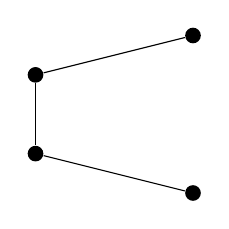
\begin{tikzpicture}[baseline=(current bounding box.north)]
				\node (v1) at (0,1) [circle,fill,inner sep=2pt] {};
				\node (v2) at (0,0) [circle,fill,inner sep=2pt] {};
				\node (v3) at (2,1.5) [circle,fill,inner sep=2pt] {};
				\node (v4) at (2,-0.5) [circle,fill,inner sep=2pt] {};
				
				\draw (v1) -- (v2);
				\draw (v1) -- (v3);
				\draw (v2) -- (v4);
			\end{tikzpicture}
			\caption{Spanning tree with 4 vertices}
		\end{subfigure}
		\hfill
		\begin{subfigure}[b]{0.4\textwidth}
			\centering
			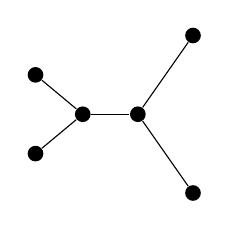
\begin{tikzpicture}[baseline=(current bounding box.north)]
				\node (v1) at (0,1) [circle,fill,inner sep=2pt] {};
				\node (v2) at (0,0) [circle,fill,inner sep=2pt] {};
				\node (v3) at (2,1.5) [circle,fill,inner sep=2pt] {};
				\node (v4) at (2,-0.5) [circle,fill,inner sep=2pt] {};
				\node (s1) at (0.6,0.5) [circle,fill,inner sep=2pt] {};
				\node (s2) at (1.3,0.5) [circle,fill,inner sep=2pt] {};
				
				\draw (v1) -- (s1);
				\draw (v2) -- (s1);
				\draw (v3) -- (s2);
				\draw (s1) -- (s2);
				\draw (v4) -- (s2);
			\end{tikzpicture}
			\caption{Steiner tree with additional points}
		\end{subfigure}
	\end{figure}

	
	\subsection{LED trees}
		-intro
	
		A special type of tree is rooted tree, a rooted tree is a tree\(G = (V , E, R)\) in which one vertex \( R \in V \) has been designated the root.A Euclidean rooted tree can be defined as a pair \( \Psi = (G, \psi) \), where \( G \) is a rooted tree and \( \psi : V \to \mathbb{R}^n \) is an arbitrary map. The vertices of \( \Psi \) are the images of the elements of \( V \), and the role of the root is naturally assigned to the vertex \( \psi(R) \). Since \( \mathbb{R}^n \) is equipped with its standard metric, we can measure the length of any edge of \( \Psi \) by evaluating the distance between its adjacent vertices.
		
		\begin{itemize}
			\item A \emph{leaf} of a tree is any vertex of degree one (with just one adjacent edge). Any other vertex is called an \emph{inner vertex}.
			\item The \emph{root path} of a vertex of a rooted tree is the unique path that connects the vertex with the root.
			\item The \emph{depth} of a vertex in a rooted tree is the length of its root path. In the non-Euclidean case, this is simply the number of edges in the path, while in the Euclidean case, the depth is the standard Euclidean length of the path.
			\item A \emph{leaf path} is any downward path that connects a vertex with a leaf. A \emph{downward path} is any path where each vertex has a greater depth than its predecessor.
			\item The \emph{height} of a vertex is the length of its longest leaf path. The \emph{height of the tree} is defined as the height of the root.
			\item The \emph{parent} of a vertex is its successor on the root path. A \emph{child} of a vertex is its successor on any of its leaf paths.
		\end{itemize}
		
		
		-some descrition (drz sa clanku L-M LEDtrees)
		
	\subsection{Relaxed LED trees}	
	
		- treba vysvetlit pojmy relaxovania a natahoania lebo s nimi pracujes v pravej sekcii o led s 3 listami
			\\
		
		% presunute z kapitoly 2 a zovseobecnene
				
		For every edge connecting two vertices in a tree, we assign two values:
		\begin{itemize}
			\item \( |uv| \): the Euclidean distance between the two vertices \( u \) and \( v \),
			\item \( \Price{u}{v} \): the relaxed (or curved) value of the edge between \( u \) and \( v \),
		\end{itemize}
		where \( |uv| \leq \Price{u}{v} \) for every edge.
		
		We will also denote \( \Price{u}{v} \) for vertices \( u \) and \( v \) that are not directly connected by an edge. In this case, \( \Price{u}{v} \) represents the sum of relaxed values along the unique path from \( u \) to \( v \). Since a tree contains no cycles, there exists exactly one such path for every pair of vertices.
		
		% tu neviem ci mam pisat takto alebo je v clanku L-M LEDtrees
		\begin{definition}\label{def:led}
			A tree is called a relaxed LED (Leaves of Equal Depth) tree if the price of the path from the root \( R \) to each leaf is the same. That is, for any two leaves \( l_1 \) and \( l_2 \), it holds that
			\[
			\Price{R}{l_1} = \Price{R}{l_2}.
			\]
		\end{definition}
	
		In other words, for any two leaves \( l_1 \) and \( l_2 \):
		\[
		 \sum_{(u,v) \in M_1} \Price{u}{v} = \sum_{(u,v) \in M_2} \Price{u}{v},
		\]
		where \( M_1 \) and \( M_2 \) are the sets of edges of paths from the root \( R \) to the leaves \( l_1 \) and \( l_2 \), respectively. The sums are taken over all edges \( (u,v) \) along the corresponding paths.
		
		From the definition of relaxed LED trees, we obtain a relation that we will find useful later.
		\begin{lemma}\label{lem:led}
			% musi byt povedane ze listy su obe za V
			Let \( V \) be a vertex that is neither a leaf nor a root, and let \( L_1 \) and \( L_2 \) be leaves. Assume that \( V \) is a common ancestor of both leaves \( L_1 \) and \( L_2 \).
			If the root \( R \) does not lie on either of the paths from \( V \) to \( L_1 \) or from \( V \) to \( L_2 \), then:
			\[
			\Price{V}{L_1} = \Price{V}{L_2}.
			\]			
		\end{lemma}
		\begin{proof}
			Let \(N\) be the path consisting of edges \((v_i, v_{i+1})\), where \(v_0 = R\) and \(v_k = V\).
			Let \(M'_1\) be the path consisting of edges \((v_i, v_{i+1})\), where \(v_0 = V\) and \(v_k = L_1\).
			Let \(M'_2\) be the path consisting of edges \((v_i, v_{i+1})\), where \(v_0 = V\) and \( v_k = L_2\).
			Define \( M_1 = N \cup M'_1 \) and \( M_2 = N \cup M'_2 \).\\
			Since the prizes along the paths from \( R \) to \( L_1 \) and \( R \) to \( L_2 \) are equal, we have:
			\begin{align*}
			\Price{R}{l_1} &= \Price{R}{l_2}\\
			\sum_{(u,v) \in M_1} \Price{u}{v} &= \sum_{(u,v) \in M_2} \Price{u}{v}\\
			\sum_{(v_i,v_{i+1}) \in N}\Price{v_i}{v_{i+1}} +\sum_{(v_i,v_{i+1}) \in M'_1}\Price{v_i}{v_{i+1}} 
			&=\sum_{(v_i,v_{i+1}) \in N}\Price{v_i}{v_{i+1}} +\sum_{(v_i,v_{i+1}) \in M'_2}\Price{v_i}{v_{i+1}}\\
			\Price{R}{V} + \Price{V}{l_1} &= \Price{R}{V} + \Price{V}{l_2} \\
			\Price{V}{l_1} &= \Price{V}{l_2}
			\end{align*}
			 For clarity, we expanded the prize terms into sums here.  
			 However, in the rest of the text, we will write prize values without explicitly unfolding the paths.
		\end{proof}
			
		We define the price of tree \(\Ptotal{T}\) as the sum of all individual \(\Price{}{}\) values.
	
	LED (leaves of equal depth)

	
	
	%--------------------------------------------------------------------------------------------
	\maketitle

	\section*{Case of 3 leaves}
	
	
	 
	\subsection{Fermat problem}
	
	
	
	\subsection{minimal relaxed LED tree with 3}
	
	Analyzing the Fermat problem provides a glimpse into the world of Steiner trees and helps us better understand the behavior of more complex Steiner trees through trivial case. Our motivation in this section is the same. We will compose a relaxed LED tree that is the most similar to one in Fermat problem and will in detail look at behaviour and properties of this structure. The structure of our relaxed LED tree is as follows:
	
	Let \( T \) be a relaxed LED tree that contains exactly three vertices \( A \), \( B \), and \( C \) of degree one (i.e., leaves), exactly one vertex \( S \) of degree three, and one vertex \( R \) of degree two (i.e., the root). Vertex \( S \) is adjacent to two leaves and to the root \( R \), while the remaining leaf is adjacent directly to the root \( R \). Every edge has price value \(\Price{u}{v}; |uv| \leq \Price{u}{v} \) and according to \cref{def:led}: 
	\[
	\Price{R}{A} = \Price{R}{B} = \Price{R}{C}
	\] 
	%obrazok
	
	In the following steps, we will focus on minimizing the total prize \(\Ptotal{T}\).
	
	
	% 0. -------------------------------------------------------------------------------
	
	since we want to minimize then tree the R must lie on one of the edges AS, BS, CS 
	
	
	
	% 1. -------------------------------------------------------------------------------
	
	
	First, given the full geometry of the LED tree, we will analyze which price function \Price{}{}, minimize its price.
	First we will analyze which edges of the tree we can tighten:
	
	For tree \( T \), we have three options how to arrange the edges, depending on which vertex other than vertex S is Root \( R \) adjacent to. Without loss of generality, assume that \(R\) is adjacent to \(C\). Which means that edges for this particular tree T are \((A,S),(B,S),(R,S),(R,C)\). According to  \cref{cor:led} for this topology the total price would be:
	 \begin{align*}
	 	\Ptotal{T} = \Price{A}{S} + \Price{B}{S} + \Price{C}{R} + \Price{R}{S}
	 \end{align*}
	 
	\begin{proposition}\label{prop:tp} 
		Let us distinguish four mutually exclusive case, depending on lengths of edges. Minimal prices of tree \(\Ptotal{T}\), for these cases are:
		\begin{enumerate}
		\item if \( |AS| > |BS|, |AS|+|SR| \geq |CR| \); then \(\Ptotal{T} = 2 |SR| + 3 |SA|\)
		\item if \( |AS| < |BS|, |BS|+|SR| \geq |CR| \); then \(\Ptotal{T} = 2 |SR| + 3 |SB|\)
		\item if \( |AS| > |BS|, |AS|+|SR| \leq |CR| \); then \(\Ptotal{T} = |SA| + 2 |CR|\)
		\item if \( |AS| < |BS|, |BS|+|SR| \leq |CR| \); then \(\Ptotal{T} = |SB| + 2 |CR|\)
		\end{enumerate}
	\end{proposition}
	\begin{proof}
		The second case is analogous to the first one, and the fourth case is analogous to the third. Therefore, we only prove the first and third cases.
		
		By Lemma~\ref{lem:led}, we know that in all cases \( \Price{S}{A} = \Price{S}{B} \).
		We also know that \( |UV| \leq  $ \Price{U}{V}$ \), hence the smallest possible value for \Price{S}{A} is \(|SA|\) and for \Price{S}{R} is \(|SR|\).
		\begin{align*}	
			\Price{S}{A} = \Price{S}{B} &= |SA| \\
			\Price{S}{R} &= |SR| \\
			\Price{R}{C} = \Price{R}{S} + \Price{S}{A} &= |SA| + |SR|
		\end{align*}
		The total prize of three is now computed as follows:
		\begin{align*}	
			\Ptotal{T} &= \Price{S}{A} + \Price{S}{B} + \Price{C}{R} + \Price{R}{S} \\
			&= |SA| + |SA| + |SR| + |SA| + |SR| \\
			&= 2 |SR| + 3 |SA|
		\end{align*}
	
		Let us analyze the third case where \( |AS| > |BS|, |AS|+|SR| \leq |CR| \).
		We know that:
		\begin{align*}
			\Price{S}{A} = \Price{S}{B}
		\end{align*}
		also that smallest possible value for \Price{S}{A} is \(|SA|\).
		\begin{align*}	
			\Price{S}{A} = \Price{S}{B} = |SA| \\
		\end{align*}
		since \(|CR| \geq |AS|+|SR| > |BS|+|SR| \), the smallest possible value for \Price{R}{C} is \(|CR|\)
		\begin{align*}
		 	\Price{R}{C} &= \Price{R}{A} = \Price{R}{B} = |CR| \\
		 	\Price{R}{C} &= \Price{R}{S} + \Price{S}{A} \\
		 	\Price{R}{S} &= |CR| - |AS|
		\end{align*}
		The total prize of three is then computed as follows:
		\begin{align*}	
			\Ptotal{T} &= \Price{S}{A} + \Price{S}{B} + \Price{C}{R} + \Price{R}{S} \\
			&= |SA| + |SA| + |CR| + |CR| - |SA| \\
			&= |SA| + 2 |CR|
		\end{align*}
	\end{proof}	 
		 
	% 2. -------------------------------------------------------------------------------	 
	
		 
	
	
	We have not yet considered the case where \( |AS| = |BS| \). Let us take a closer look at it. 
	
	First, we assume that \( |AS| + |SR| > |CR| \) and \( |BS| + |SR| > |CR| \), and let \( |SR| \) be a fixed distance.
	\begin{align*}
		|AS| = |BS| = d, \quad d \in R \\
		\Ptotal{T_1} = 2|SR| + 3|SA| = 2|SR| + 3|BS| = 2|SR| + 3d
	\end{align*}
	Now suppose that \( |AS| = d + k \), where \( k > 0 \). Then the total prize becomes:
	\[
	\Ptotal{T_2} = 2|SR| + 3(d + k) = 2|SR| + 3d + 3k > \Ptotal{T_1}
	\]
	Similarly, if \( |BS| = d + k \), we have:
	\[
	\Ptotal{T_3} = 2|SR| + 3(d + k) = 2|SR| + 3d + 3k > \Ptotal{T_1}
	\]
	In both cases, when either \( |AS| \) or \( |BS| \) deviates from \( d \), the total length of the tree increases compared to the symmetric case. It follows that the minimal total length is achieved when \( |AS| = |BS| \).
	
	Now consider the second case, where \( |AS| + |SR| \leq |CR| \) and \( |BS| + |SR| \leq |CR| \), and let \( |CR| \) be fixed:
	\begin{align*}
		|AS| = |BS| = d, \quad d \in R \\
		L(T_1) = 2|CR| + |SA| = 2|CR| + |SB| = 2|CR| + d
	\end{align*}
	Now suppose that \( |AS| = d + k \), where \( k > 0 \). Then the total length becomes:
	\[
	L(T_2) = 2|CR| + d + k > L(T_1)
	\]
	If \( |BS| = d + k \), we have:
	\[
	L(T_3) = 2|CR| + d + k > L(T_1)
	\]
	Again, it is clear that the minimal total length is achieved when \( |AS| = |BS| \).\\

	Now let us analyze the case when \(|AS|+|SR| = |CR| \).
	The total length would be \[ L(T) = |SA| + 2 |CR| = L(T) = |AS| + 2|AS| + 2|SR| = 3|AS| + 2|SR|  )\]
	Let \( d > 0 \) and suppose we fix \( |CR| \) and \( |SR| \), and increase \( |AS| \) by \( d \):
	\[
	|AS|^* = |AS| + d \quad \Rightarrow \quad L(T_1) = 2|SR| + 3|AS|^* = 2|SR| + 3(|AS| + d) = L(T) + 3d > L(T)
	\]
	
	Now fix \( |CR| \) and \( |AS| \), and increase \( |SR| \) by \( d \):
	\[
	|SR|^* = |SR| + d \quad \Rightarrow \quad L(T_2) = 2|SR|^* + 3|AS| = 2(|SR| + d) + 3|AS| = L(T) + 2d > L(T)
	\]
	
	Now fix \( |SR| \) and \( |AS| \), and increase \( |CR| \) by \( d \):
	\[
	|CR|^* = |CR| + d \quad \Rightarrow \quad L(T_3) = |AS| + 2|CR|^* = |AS| + 2(|CR| + d) = L(T) + 2d > L(T)
	\]
	
	In all cases, any deviation from the equality \( |AS| + |SR| = |CR| \) leads to an increase in the total length.  
	Therefore, the minimal total length of the tree is achieved exactly when
	\[
	|AS| + |SR| = |CR|
	\]
	A completely analogous argument applies when \( |BS| + |SR| = |CR| \).  
	Again, increasing \( |BS| \), \( |SR| \), or \( |CR| \) individually while keeping the others fixed leads to an increase in the total length.  
	Hence, the minimal total length is achieved exactly when:
	\[
	|BS| + |SR| = |CR|
	\]
	
	
	This leads us to the question of how to place the root \( R \in \overline{CS} \) for given points \( A, B, C, S \), so that the total length of the LED tree is minimized. From the constraint \( |AS|+|SR| = |CR|  \), we derive:
	
	\begin{align*}
		|AS| + |CS| &= |AS| + |SR| + |RC| \\
		|AS|+|CS| &= |AS|+|SR|+|AS|+|SR| \\ 
		|CS| &= |AS|+2|SR| \\
		|SR| &= \frac{|CS| - |AS|}{2} \\
		\Rightarrow \quad |RC| &= |CS| - |SR| = |CS| - \frac{|CS| + |AS|}{2}
	\end{align*}
	Therefore, to minimize the total length of the LED tree, the root \( R \) should be placed on edge \( \overline{CS} \) such that its distance from \( S, C\) is:
	\[
	|SR| = \frac{|CS| - |AS|}{2},  |RC| = |CS| - \frac{|CS| + |AS|}{2}
	\]
	
	Assume \( |AS| < |BS| < |CS| \) and suppose, for contradiction, that the root \( R \) lies on edge \( \overline{BS} \).  
	Let us assume that the minimal LED tree satisfies:
	\[
	\Price{R}{C} = \Price{R}{B} = \Price{R}{A}
	\]
	Then in particular:
	\[
	\Price{R}{C} = \Price{R}{S} + \Price{S}{C} = \Price{R}{B} = |BR|
	\]
	
	Now since \( R \in \overline{BS} \), we have \( |BR| < |BS| \), and from the assumption above:
	\[
	|SR| + |CS| = |BR| < |BS| < |CS|
	\quad \Rightarrow \quad |SR| < 0
	\]
	
	which is a contradiction.  
	The same argument applies if \( R \in \overline{AS} \).  
	Therefore, the only edge that avoids contradiction is the longest one, i.e. \( \overline{CS} \).  
	Hence, to minimize the total length while satisfying the LED condition, the root must lie on the longest edge from \( S \).
	
	
	\end{document}
